\chapter{METODOLOGI}

% Ubah konten-konten berikut sesuai dengan isi dari metodologi

Dalam upaya mencapai tujuan penelitian yang terkait dengan penelitian yang berjudul Prediksi Semaphore berbasis \textit{Deep Learning }, metode penelitian yang telah direncanakan telah dijabarkan dalam Gambar \ref{fig:blokdiagram}. Rangkaian metode yang sudah disusun ini mencakup beberapa tahapan yang akan diuraikan secara rinci .

\section{Block Diagram Penelitian}
Adapun alur dari penelitian ini dapat dilihat pada Gambar \ref{fig:blokdiagram}.
\begin{figure}[hbt!]
	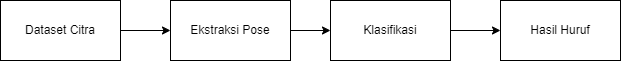
\includegraphics[width=1.0\linewidth]{gambar/metodologi_kerja.png}
	\captionof{figure}{Blok Diagram Penelitian}
	\label{fig:blokdiagram}
\end{figure}
Penjelasan mengenai \textit{Block Diagram} secara rinci dan detail akan disajikan pada sub-sub bab berikutnya. Penyajian informasi dalam bentuk \textit{Block Diagram} menjadi salah satu langkah penting dalam menggambarkan struktur dan alur dari sistem atau proses yang dijelaskan dalam penelitian ini. \textit{Block Diagram} menyediakan gambaran visual yang jelas dan sistematis tentang bagaimana berbagai komponen atau elemen dalam sistem saling berhubungan dan berinteraksi satu sama lain.

\section{Dataset Citra}
Penelitian ini mengadopsi sebuah dataset citra yang sangat beragam dan informatif, terdiri dari total 26 huruf alfabet serta satu Huruf Akhir yang sering dijumpai dalam berbagai situasi kehidupan sehari-hari seperti pada Gambar \ref{fig:poseAbjadBISINDO}. Dataset yang digunakan ini menjadi pilar utama dalam proses pelatihan dan pengujian model yang sedang dikembangkan dalam konteks penelitian ini. Data citra yang beragam ini akan memberikan informasi yang lebih lengkap dan representatif agar membantu menghasilkan hasil yang lebih kuat dan reliabel dalam pengujian model tersebut.
\begin{figure}[hbt!]
	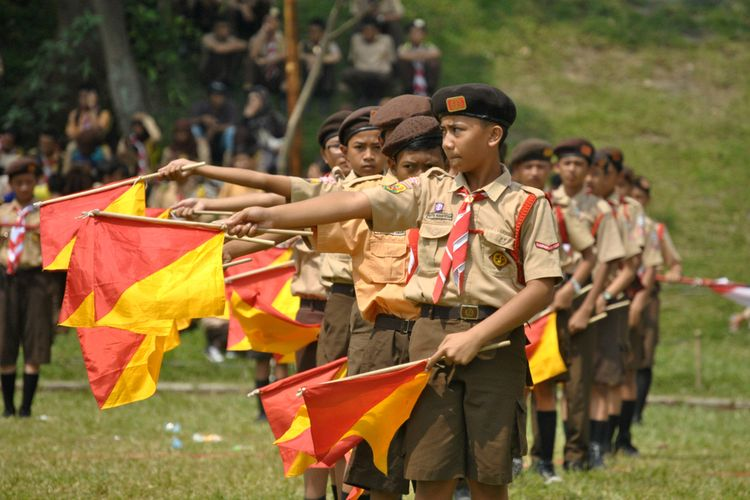
\includegraphics[width=0.7\linewidth]{gambar/bener/kerja-semaphore.jpg}
	\captionof{figure}{Contoh Pose Semaphore}
	\label{fig:poseAbjadBISINDO}
\end{figure}
Penelitian ini memanfaatkan sebuah dataset citra yang terdiri dari jumlah yang sangat signifikan yaitu 26.000 citra secara keseluruhan. Setiap huruf alfabet, sebanyak 26 huruf, diwakili oleh tak kurang dari 1000 citra yang khusus dipilih mewakili masing-masing huruf tersebut. Dengan total 26.000 citra yang teliti dan cermat ini, dataset menjadi sangat beragam dan mendalam, menyediakan beragai representasi visual setiap huruf. Hal ini bertujuan memberikan kesempatan kepada model yang sedang dikembangkan mengenali dan memprediksi huruf-huruf ini dengan tingkat akurasi yang tinggi. Proses pelatihan dan pengujian model dengan menggunakan dataset sebesar ini diharapkan akan menghasilkan kemampuan model yang lebih canggih dan unggul dalam pengenalan huruf dalam citra.
\section{Ekstraksi Pose}
Proses Ekstraksi Pose merupakan tahap penting dalam pengolahan data pada dataset Gambar 3.2 . Dalam proses ini, digunakan teknologi machine learning bernama \textit{MediaPipe} yang dikembangkan oleh Google menghasilkan skeleton yang merepresentasikan pose tubuh pada setiap gambar. Agar memudahkan pembacaan oleh model, latar belakang gambar diubah menjadi seragam berwarna hitam. \textit{MediaPipe} memungkinkan deteksi gerakan pose dengan efisien. Dalam proses ini, dilakukan ekstraksi fitur dari skeleton pose yang disediakan oleh \textit{MediaPipe}. Namun, dalam pengerjaan ini, hanya beberapa bagian penting dari  pose yang digunakan, sesuai dengan yang ditampilkan pada Gambar \ref{fig:CITRAAWAL1}
\begin{figure}[hbt!]
	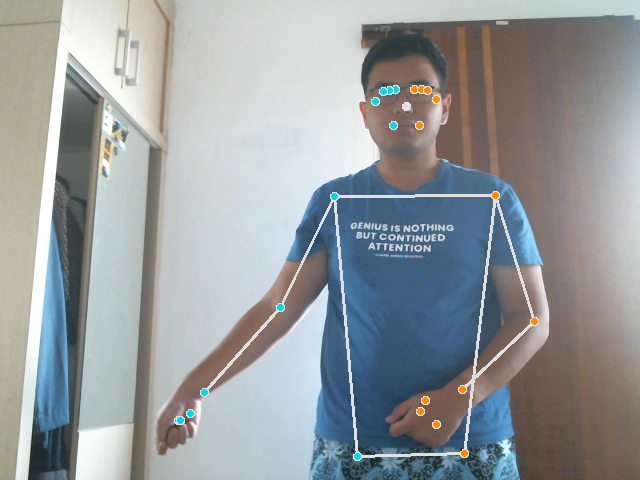
\includegraphics[width=0.7\linewidth]{gambar/Gambar3.3.png}
	\captionof{figure}{Hasil Estimasi Pose dengan MediaPipe}
	\label{fig:CITRAAWAL1}
\end{figure}
Selanjutnya, program yang dikembangkan pada penelitian ini akan mengekstraksi skeleton \textit{MediaPipe} dari Gambar \ref{fig:CITRAAWAL1} dan mengganti semua aspek gambar dataset dengan latar hitam, seperti terlihat pada Gambar \ref{fig:CITRAAKHIR1}.
\begin{figure}[hbt!]
	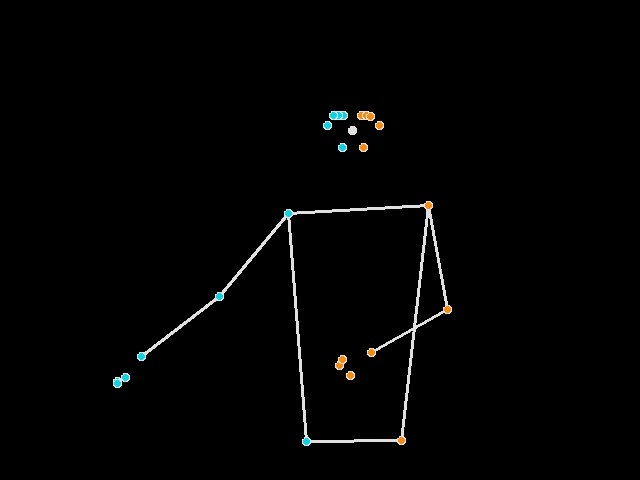
\includegraphics[width=0.7\linewidth]{gambar/Gambar3.4.jpg}
	\captionof{figure}{Hasil Estimasi Pose Siluet: Data Latih Deteksi Gerakan Tubuh}
	\label{fig:CITRAAKHIR1}
\end{figure}
Dengan melakukan ekstraksi pose ini, diharapkan dapat menggambarkan pose tubuh secara akurat pada setiap gambar dalam dataset. Hal ini menjadi dasar penting dalam pengembangan model dan analisis selanjutnya, serta memungkinkan pengenalan pola gerakan yang terkait dengan bagian-bagian penting pada tubuh bagian atas. Berikut ini merupakan tabel dari bagian pose yang digunakan dan dikelompokkan kedalam kelompok \textit{Upper Body Connection}
\begin{center}
	\begin{table}[hbt!]
		\captionof{table}{Pose Landmarks}
		\label{tbl:PoseLandmarks}
		\centering
		\begin{tabular}{cc}
			\hline
			Nomor & Nama Bagian \\
			\hline
			
			11 & Left Shoulder \\
			\hline
			
			12 & Right Shoulder \\
			\hline
			
			13 & Left Elbow \\
			\hline
			
			14 & Right Elbow \\
			\hline
			
			15 & Left Wrist \\
			\hline
			
			16 & Right Wrist \\
			\hline
			
			23 & Left Hip \\
			\hline
			
			24 & Right Hip \\
			\hline
		\end{tabular}
	\end{table}
	\end{center}
\section{Klasifikasi Pose}
Pada tahapan ini akan dilakukan proses klasifikasi dari data yang sudah melewati tahap estimasi dan esktrimasi \textit{skeleton} dan \textit{landmarks} yang sudah disediakan dari \textit{\textit{MediaPipe}} . Lalu dalam tahapan ini  diterapkan \textit{Convolutional Neural Network} supaya dilatih dan juga disini bisa didapatkan hasil klasifikasi dari huruf yang sudah diperagakan

\subsection{Metode CNN}
Model \textit{CNN} sesuai dengan Gambar \ref{fig:layerCNN} menggunakan beberapa lapisan konvolusi dan lapisan \textit{pooling} mengekstraksi fitur-fitur penting dari gambar. Input gambar memiliki dimensi 128x128 dengan 3 saluran warna \textit{(RGB)}. Kemudian, dilakukan konvolusi dengan 32 ,32 , 32 , 16 \textit{filter} berukuran 3x3 dan aktivasi \textit{ReLU}. Lapisan konvolusi ini bertujuan mengekstraksi fitur-fitur visual pada gambar. Setelah itu, dilakukan proses \textit{pooling} dengan menggunakan lapisan \textit{MaxPooling2D} dengan ukuran \textit{filter} 2x2. \textit{Maxpooling} digunakan mereduksi dimensi fitur dan mempertahankan fitur yang paling signifikan.
\begin{figure}[hbt!]
	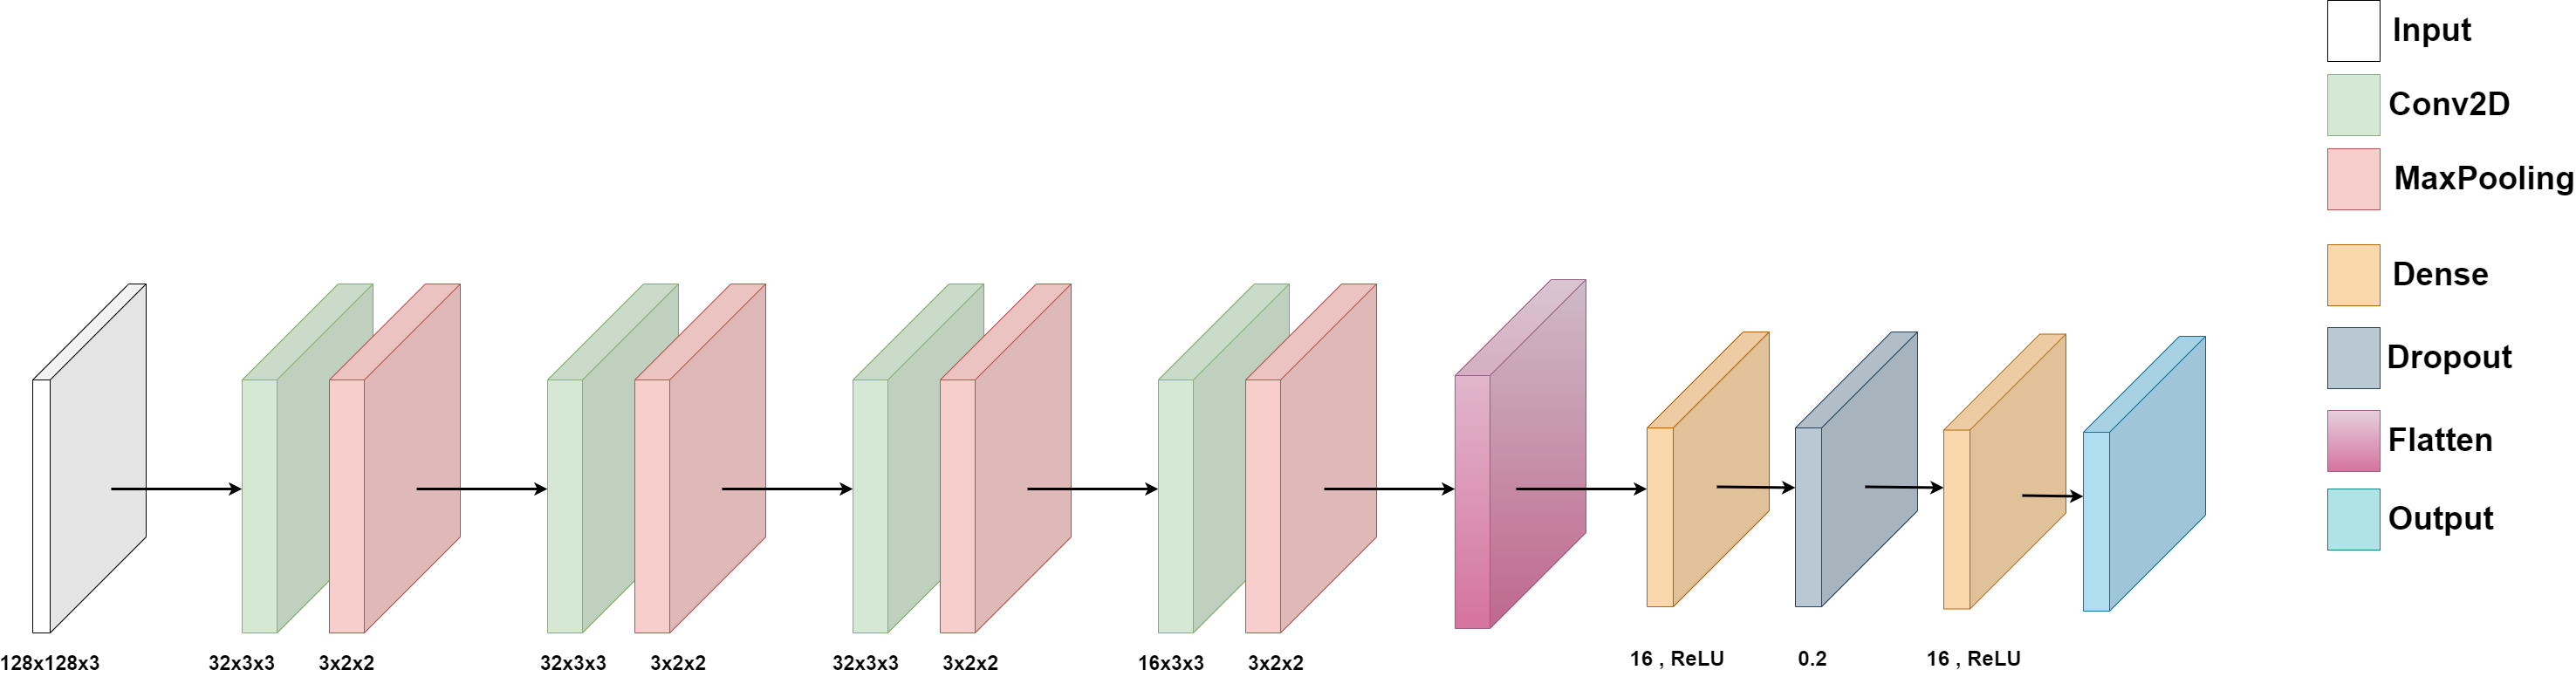
\includegraphics[width=1.0\linewidth]{gambar/bener/Arsitektur_CNN_Revisi.png}
	\captionof{figure}{Layers dari Model CNN}
	\label{fig:layerCNN}
\end{figure}
Langkah-langkah konvolusi dan \textit{pooling} ini diulangi beberapa kali meningkatkan representasi fitur secara bertahap. Setelah serangkaian konvolusi dan \textit{pooling}, terdapat lapisan \textit{Flatten} meratakan fitur-fitur spasial menjadi vektor fitur satu dimensi.Selanjutnya, terdapat dua lapisan \textit{{Dense} (fully connected)} berturut-turut dengan aktivasi \textit{ReLU}. Lapisan ini bertujuan memperkenalkan non-linearitas dan mempelajari hubungan antara fitur-fitur yang diekstraksi.

Lapisan \textit{Dropout} dengan tingkat \textit{dropout} 0.2 diterapkan menghindari \textit{overfitting} dengan secara acak "menonaktifkan" sebagian unit dalam lapisan tersebut. Terakhir, terdapat lapisan {\textit{Dense}} dengan jumlah unit sebanyak JumlahKelas, yang sesuai dengan jumlah kelas yang akan diprediksi oleh model. Lapisan ini menggunakan aktivasi \textit{softmax}, yang menghasilkan distribusi probabilitas setiap kelas. Seluruh model ini diinisialisasi menggunakan objek Model dari \textit{Keras}, dengan input gambar sebagai input dan lapisan terakhir sebagai output. Model ini dikompilasi menggunakan \textit{optimizer Adam} dan \textit{loss function} berupa \textit{mean squared error (MSE)}, yang sering digunakan tugas regresi. Metrik akurasi juga digunakan mengukur performa model.

\subsection{Metode CNN Kedua}
Model \textit{CNN} inilah yang menggunakan beberapa lapisan konvolusi dan lapisan \textit{pooling} mengekstraksi fitur-fitur penting dari gambar. Gambar input memiliki dimensi $128 \times 128$ dengan 3 saluran warna \textit{(RGB)}. Kemudian, konvolusi dilakukan menggunakan 32, 16, 16, dan 8 \textit{filter} berukuran $3 \times 3$ dengan aktivasi \textit{ReLU}. Lapisan konvolusi bertujuan mengekstraksi fitur-fitur visual pada gambar.

Selanjutnya, dilakukan \textit{pooling} dengan menggunakan lapisan \textit{MaxPooling2D} dengan ukuran \textit{filter} $2 \times 2$. Max \textit{pooling} digunakan mereduksi dimensi fitur dan mempertahankan fitur yang paling signifikan.

\begin{figure}[hbt!]
	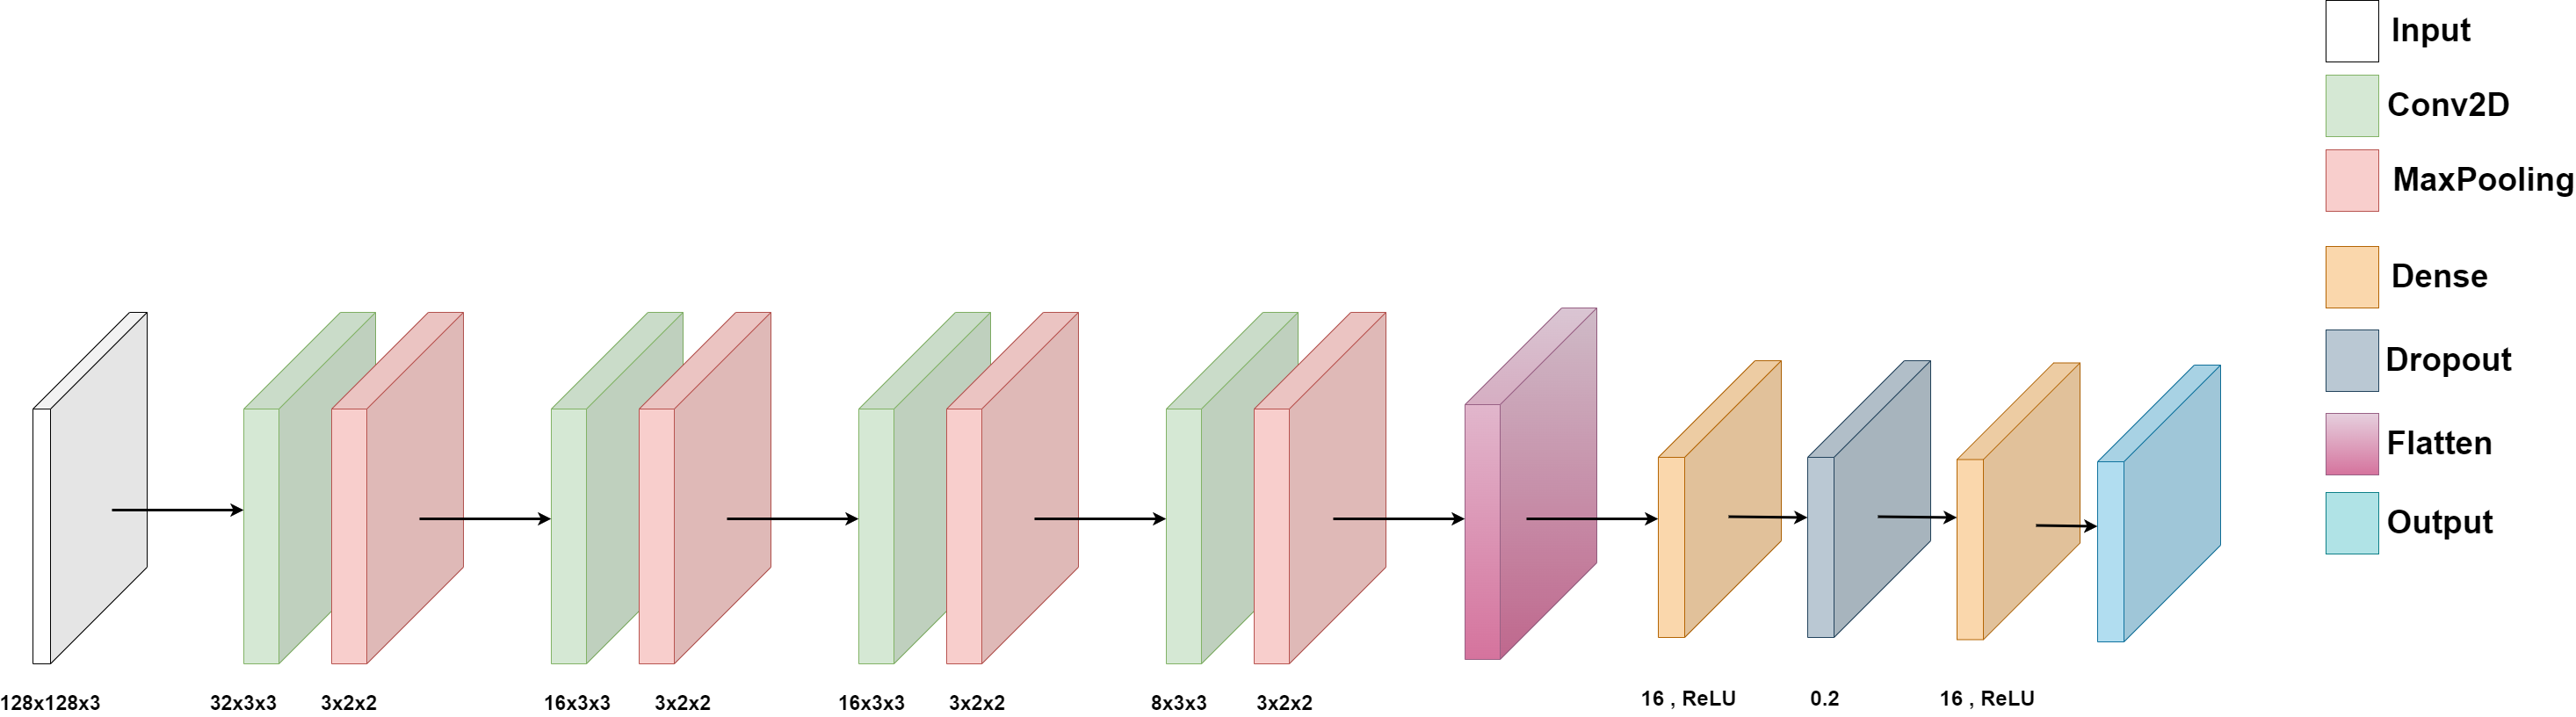
\includegraphics[width=1.0\linewidth]{gambar/bener/Arsitektur_CNN2_Revisi.png}
	\captionof{figure}{Layers dari Model CNN Kedua}
	\label{fig:layerCNN}
\end{figure}

Proses konvolusi dan \textit{pooling} ini diulangi beberapa kali meningkatkan representasi fitur secara bertahap. Setelah serangkaian konvolusi dan \textit{pooling}, terdapat lapisan \textit{Flatten} meratakan fitur-fitur spasial menjadi vektor fitur satu dimensi.Selanjutnya, terdapat dua lapisan \textit{Dense} (fully connected) berturut-turut dengan aktivasi \textit{ReLU}. Lapisan ini bertujuan memperkenalkan non-linearitas dan mempelajari hubungan antara fitur-fitur yang diekstraksi. Lapisan \textit{Dropout} dengan tingkat \textit{dropout} 0.2 diterapkan dalam menghindari \textit{overfitting} dengan secara acak "menonaktifkan" sebagian unit dalam lapisan tersebut.

Terakhir, terdapat lapisan \textit{Dense} dengan jumlah unit sebanyak JumlahKelas, yang sesuai dengan jumlah kelas yang akan diprediksi oleh model. Lapisan ini menggunakan aktivasi \textit{softmax}, yang menghasilkan distribusi probabilitas setiap kelas. Seluruh model ini diinisialisasi menggunakan objek \textit{Model} dari Keras, dengan input gambar sebagai input dan lapisan terakhir sebagai output. Model ini dikompilasi menggunakan optimizer \textit{Adam} dan \textit{loss function} berupa \textit{mean squared error (MSE)}, yang sering digunakan oleh tugas regresi. Metrik akurasi juga digunakan mengukur performa model.

\subsection{Metode CNN Xception}
Arsitektur pada Gambar \ref{fig:Xception} adalah sebuah model \textit{Convolutional Neural Network (\textit{CNN})} yang menggunakan arsitektur \textit{Xception} sebagai bagian dasarnya. \textit{Xception} adalah salah satu model \textit{CNN} yang dikembangkan oleh François Chollet sebagai bagian dari library Keras. Pada arsitektur ini, input gambar memiliki dimensi 128x128 dengan 3 saluran warna \textit{(RGB)}. Kemudian, model \textit{Xception} yang telah dilatih sebelumnya pada dataset \textit{ImageNet} digunakan sebagai bagian dasar dari model. Model \textit{Xception} ini diinisialisasi dengan bobot yang telah diatur oleh pelatihan pada \textit{ImageNet}.Selanjutnya, seluruh lapisan di dalam model \textit{Xception} dibekukan \textit{(frozen)} atau tidak akan diperbarui selama pelatihan. Hal ini dilakukan dengan tujuan mempertahankan pengetahuan yang telah dipelajari oleh model \textit{Xception} dari dataset \textit{ImageNet}.

\begin{figure}[hbt!]
	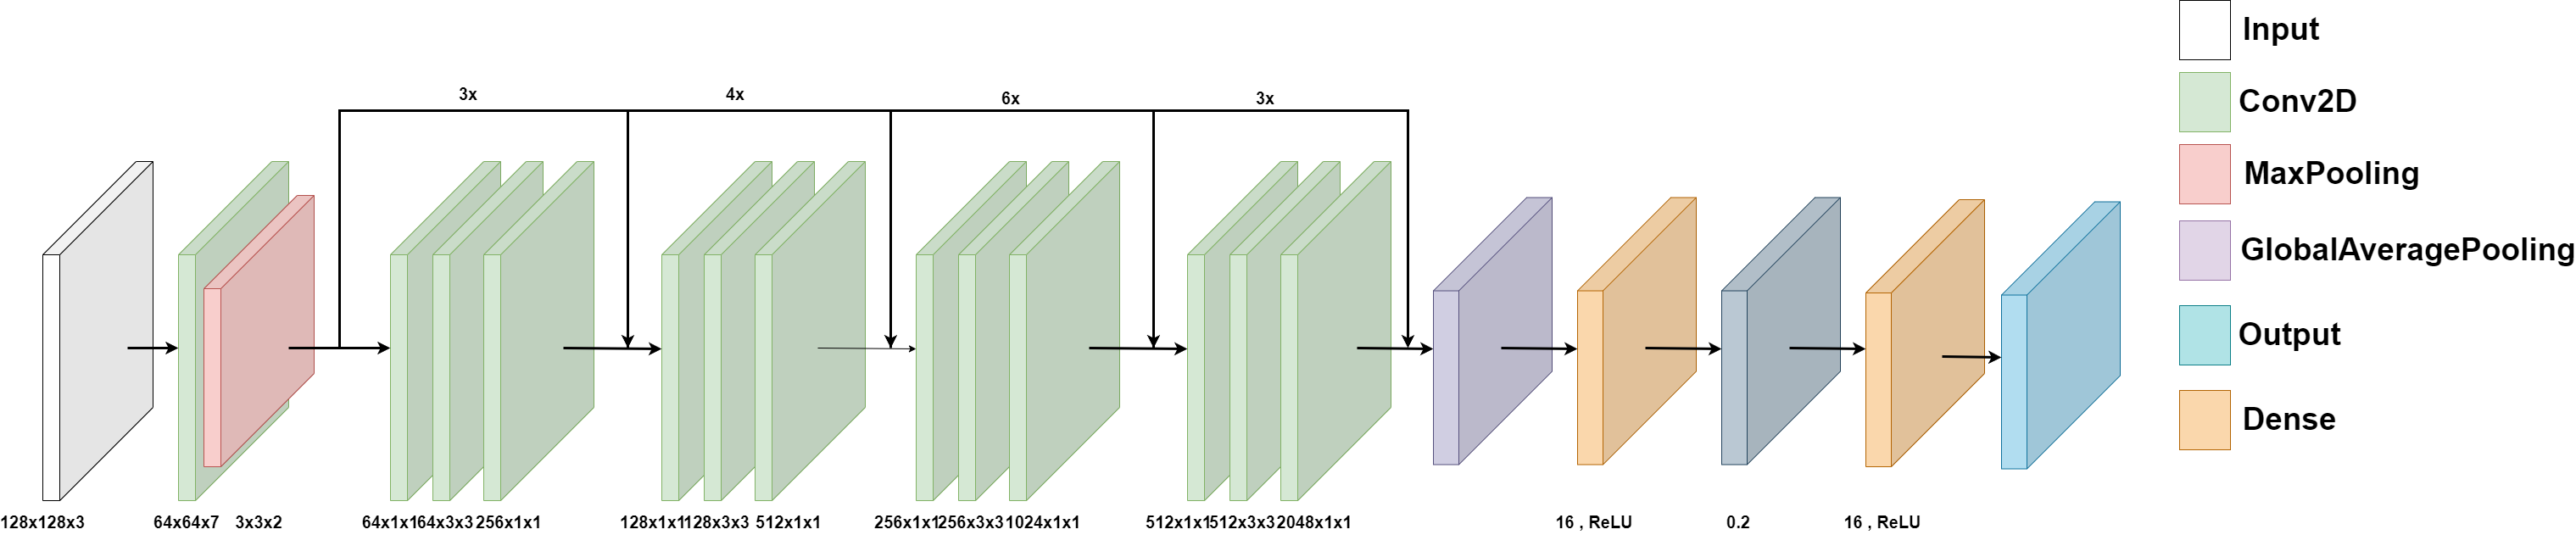
\includegraphics[width=1.0\linewidth]{gambar/bener//Arsitektur_CNNXception_Modifikasi.png}
	\captionof{figure}{Layers dari Model CNN  Xception}
	\label{fig:Xception}
\end{figure}
Setelah itu, keluaran (output) dari model \textit{Xception} dihubungkan ke lapisan Flatten yang berfungsi meratakan fitur-fitur spasial menjadi vektor fitur satu dimensi. Kemudian, terdapat tiga lapisan \textit{Dense (fully connected)} berturut-turut dengan aktivasi \textit{ReLU}.Pada lapisan pertama \textit{Dense} dengan 16 unit, aktivasi \textit{ReLU} digunakan memperkenalkan non-linearitas. Kemudian, diterapkan \textit{Dropout} dengan tingkat \textit{dropout} sebesar 0.2, yang berfungsi menghindari \textit{overfitting} dengan secara acak "menonaktifkan" sebagian unit dalam lapisan tersebut.

Selanjutnya, dilanjutkan dengan lapisan \textit{Dense} kedua dengan 16 unit dan aktivasi \textit{ReLU}. Lapisan ini juga memiliki tujuan memperkenalkan non-linearitas dan menghasilkan representasi fitur yang lebih kompleks. Terakhir, terdapat lapisan \textit{Dense} dengan jumlah unit sebanyak JumlahKelas, yang sesuai dengan jumlah kelas yang akan diprediksi oleh model. Lapisan ini menggunakan aktivasi \textit{softmax}, yang menghasilkan distribusi probabilitas setiap kelas. Seluruh model ini diinisialisasi menggunakan objek Model dari Keras, dengan input gambar sebagai input dan lapisan terakhir sebagai output. Model ini dikompilasi menggunakan \textit{optimizer Adam} dan \textit{loss function} berupa\textit{ mean squared error (MSE)}, yang sering digunakan tugas regresi. Selain itu, metrik akurasi juga digunakan mengukur performa model.

\subsection{Metode CNN ResNet50V2}
Pada Arsitektur \textit{ResNet50V2} sesuai Gambar \ref{fig:textitResNet50V2} , input gambar memiliki dimensi 128x128 dengan 3 saluran warna \textit{(RGB)}. Model \textit{ResNet50V2} yang telah dilatih sebelumnya pada dataset \textit{ImageNet} digunakan sebagai bagian dasar dari model. Model ini diinisialisasi dengan bobot yang telah diatur oleh pelatihan pada dataset tersebut. Selanjutnya, seluruh lapisan di dalam model \textit{ResNet50V2} dibekukan \textit{(frozen)} atau tidak akan diperbarui selama pelatihan. Hal ini dilakukan agar mempertahankan pengetahuan yang telah dipelajari oleh model \textit{ResNet50V2} dari dataset \textit{ImageNet}. Keluaran (output) dari model \textit{ResNet50V2} dihubungkan ke lapisan \textit{GlobalAveragePooling2D}, yang berfungsi merata-ratakan fitur-fitur spasial menjadi satu vektor fitur.
\begin{figure}[hbt!]
	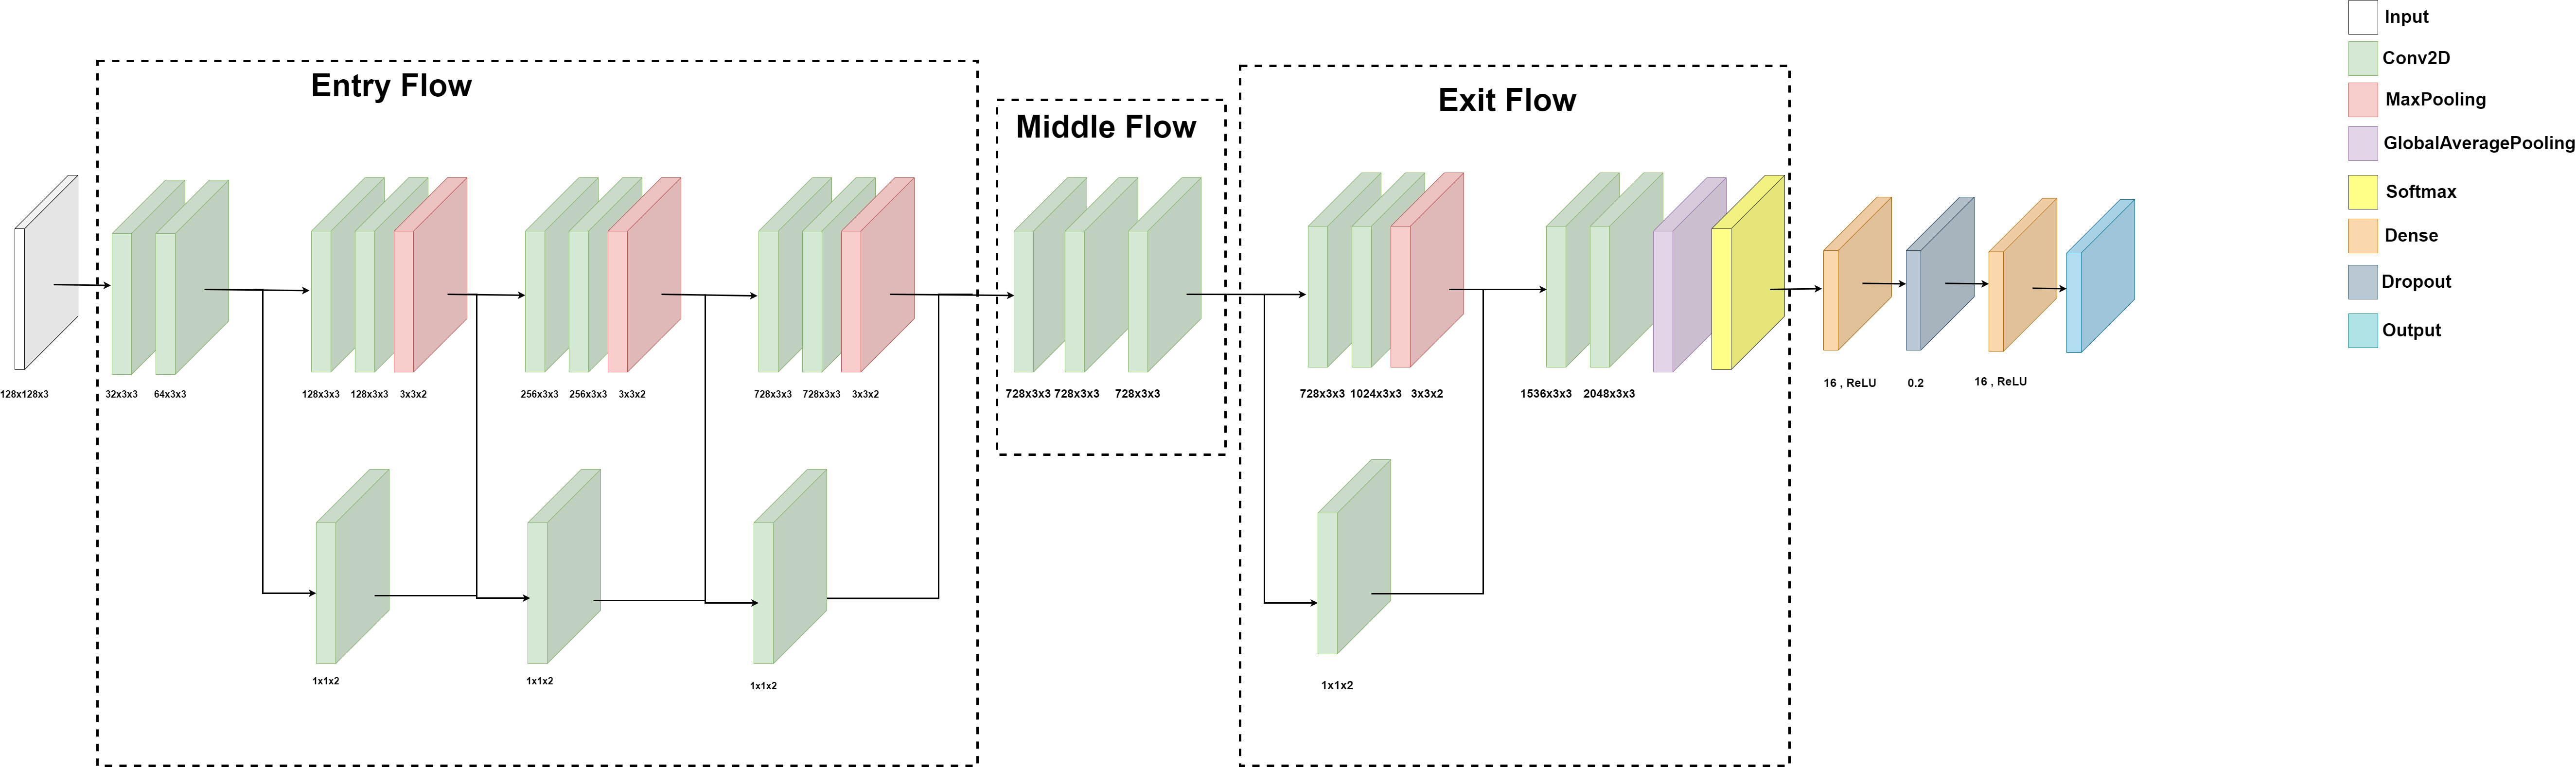
\includegraphics[width=1.1\linewidth]{gambar/bener/Arsitektur_ModelCNNResNet50v2_Modifikasi.png}
	\captionof{figure}{Layers dari Model CNN ResNet50V2}
	\label{fig:textitResNet50V2}
\end{figure}
Kemudian, terdapat tiga lapisan \textit{Dense} (fully connected) berturut-turut dengan aktivasi \textit{ReLU}. Pada lapisan pertama \textit{Dense} dengan 16 unit, aktivasi \textit{ReLU} digunakan dalam memperkenalkan non-linearitas. Lapisan \textit{Dropout} dengan tingkat \textit{dropout} sebesar 0.2 juga diterapkan mencegah \textit{overfitting} dengan secara acak "menonaktifkan" sebagian unit dalam lapisan tersebut. Lapisan \textit{Dense} kedua juga menggunakan aktivasi \textit{ReLU} dan memiliki regularisasi L2 dengan koefisien 0.01. Regularisasi L2 membantu dalam mencegah \textit{overfitting} dengan mengenakan hukuman pada bobot model yang lebih besar.

Terakhir, terdapat lapisan \textit{Dense} dengan jumlah unit sebanyak JumlahKelas, yang sesuai dengan jumlah kelas yang akan diprediksi oleh model. Lapisan ini menggunakan aktivasi \textit{softmax}, yang menghasilkan distribusi probabilitas setiap kelas. Seluruh model ini diinisialisasi menggunakan objek Model dari \textit{Keras}, dengan input gambar sebagai input dan lapisan terakhir sebagai output. Model ini dikompilasi menggunakan \textit{optimizer Adam} dan \textit{loss function} berupa\textit{ mean squared error (MSE)}, yang sering digunakan oleh tugas regresi. Selain itu, metrik akurasi juga digunakan ketika mengukur performa model.

\section{Hasil Huruf}
Hasil dari implementasi Model \textit{CNN} selanjutnya dilakukan proses pengujian dan mendapatkan citra hasil huruf . Pada tahap ini terdapat empat aspek yang dihitung yaitu akurasi, presisi, \textit{recall}, dan \emph {F-measure}. Empat aspek tersebut akan digunakan saat melihat performan dari metode yang digunakan. Adapun proses perhitungan keempat askpek tersebut dapat dilihat seperti pada Gambar \ref{fig:MATRIKSKONFUSI}.
\begin{figure}[hbt!]
	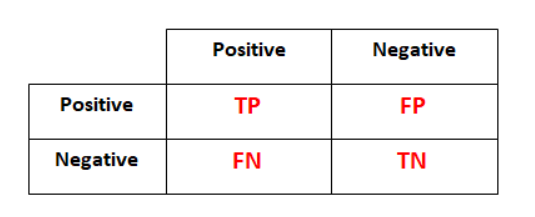
\includegraphics[width=0.7\linewidth]{gambar/bener/Nilai-Konfusi-Matriks.png}
	\captionof{figure}{Matriks konfusi}
	\label{fig:MATRIKSKONFUSI}
\end{figure}

\subsection{Akurasi}
Akurasi adalah persamaan ukuran perhitungan performa yang paling intuitif dan hanya rasio pengamatan yang diprediksi dengan benar. Sebagaimana dirumuskan dengan Persamaan (\ref{eq:persamaan1})
\begin{equation}\label{eq:persamaan1}
Akurasi=\frac{TP+TN}{TP+FP+FN+TN}
\end{equation}
\subsection{Presisi}
Presisi merupakan kecocokan antara semua bagian-bagian data yang diambil dengan informasi yang dibutuhkan. Sebagaimana dirumuskan dengan Persamaan (\ref{eq:persamaan2})
\begin{equation}\label{eq:persamaan2}
Presisi_k=\frac{TP_k}{TP_k+FP_k}
\end{equation} 
{\it Presisi Rata-rata}
\begin{equation}\label{eq:persamaan3}
Presisi \, Rata-rata=\frac{\sum_{k=1}^K Presisi_k}{K}
\end{equation} 
\subsection{Recall}
\textit{Recall} adalah tingkat keberhasilan model dalam menemukan
kembali sebuah informasi. Sebagaimana dirumuskan dengan Persamaan (\ref{eq:persamaan3})
\begin{equation}\label{eq:persamaan4}
Recall_k=\frac{TP_k}{TP_k+FN_k}
\end{equation} 
{\it Recall Rata-rata}
\begin{equation}\label{eq:persamaan5}
Recall \, Rata-rata=\frac{\sum_{k=1}^K Recall_k}{K}
\end{equation} 
\subsection{F1-Score}
\textit{F-1 Score} menggambarkan perbandingan rata-rata antara precision dan recall yang telah dibobotkan. Sebagaimana dirumuskan dengan Persamaan (\ref{eq:persamaan4})
\begin{equation}\label{eq:persamaan6}
F1-Score=2 \left( \frac{Presisi \, Rata-rata \times Recall \, Rata-rata}{Presisi \, Rata-rata^{-1} + Recall \, Rata-rata^{-1}} \right)
\end{equation} 

